\subsection{Edit Distance}
Edit distance is a measure of how many edit operations are required to convert one sequence into another.
Different edit distance measures exist, varying in the set of allowed operations.
The most common is the \emph{Levenshtein distance}~\cite{levenshtein}, allowing single character substitutions, insertions and deletions. 

Finding the edit distance between two sequences, and which set of edits this edit distance corresponds to, is of central importance in bioinformatics since it can give an estimate of how related the two sequences are and which mutations have separated them.
The process of finding these estimates is called \emph{sequence alignment} and is important for this thesis in two respects.
Firstly, it is one of the earliest and most intuitive applications of sequence graphs, and secondly it is an important part of \emph{mapping} which will be covered in the next section. 

In the following we will refer to the edit distance between two sequences, $S$ and $T$, as $D(S, T)$, here meaning the Levenshtein distance unless specifically mentioned.
The concepts discussed are however generalisable to other (weighted) edit distances and similarity measures by small changes.

The set of edits between two sequences can be represented with an \emph{alignment block} where ``-'' symbols are inserted into the sequences to represent insertions and deletions (indels), (see Figure~\ref{fig:needle}).

\subsection{Pairwise Sequence Alignment}
\label{sec:pairwise}
Finding the edit distance between two strings is easy if indels are not considered.
It is merely the process of counting the number of mismatches between them.
Indels introduce a dependency since an insertion at position $i$ affects the pairings of all the symbols after position $i$.
The number of meaningful combinations of insertions and deletions grow exponentially with sequence length, so exploring all of them is not a viable solution even for short sequences.
The problem is however tractable since the best alignment of two sequences $S[:M], T[:N]$ is either the best alignment of $S[:M-1], T[:N]$ with an insertion at the end, or of $S[:M], T[:N-1]$ with a deletion at the end, or of $S[:M-1], T[:N-1]$ with a match or substitution at the end. 
Letting $d_{i,j} = D(S[:i], T[:j])$ and $m_{i,j}$ be zero if $S[i]=T[j]$ else $1$, we can write this as the recurrence relation:
\begin{align*}
  d_{k,l} = min\begin{cases}
  &d_{k-1,l-1}+m_{k-1, l-1}\quad \text{(match/substitution)}\\
  &d_{k-1,l}+1 \quad \text{(insertion)}\\
  &d_{k, l-1}+1 \quad \text{(deletion)}\\
\end{cases}
\end{align*}
The fact that the edit distance to a empty string is just the sequence length gives the initial conditions $d_{k, 0}=k,\,d_{0,l}=l$.
The Needleman-Wunch algorithm~\cite{needlemanwunch} uses dynamic programming to calculate the matrix of edit distances $d_{kl}$, where $d_{MN}$ is the edit distance between $S[:M]$ and $T[:N]$.
In order to find the specific edits, a backtracking algorithm is used that starts at the $(i, j) = (M, N)$ corner and finds out which of the possible predecessors $(i-1, j), (i-1, j-1), (i, j-1)$ contributed to the $(i, j)$ edit distance.
Then repeating this until the $(0, 0)$ corner is reached. Each of these steps correspond to a column in the alignment block.
Figure~\ref{fig:needle} details the Needleman Wunch algorithm.
\begin{figure}
  \begin{tikzpicture}
    \matrix (m) [matrix of math nodes, align=right, row sep=0.1em,column sep=0.1em, minimum width=1em, minimum height=1em, nodes={align=right}, ]{\textcolor{red}{0} & \textcolor{black!25}{-1} & \textcolor{black!25}{-2} & \textcolor{black!25}{-3} & \textcolor{black!25}{-4} & \textcolor{black!25}{-5} & \textcolor{black!25}{-6}\\ 
\textcolor{black!25}{-1} & \textcolor{red}{0} & \textcolor{black!25}{-1} & \textcolor{black!25}{-2} & \textcolor{black!25}{-3} & \textcolor{black!25}{-4} & \textcolor{black!25}{-5}\\ 
\textcolor{black!25}{-2} & \textcolor{black!25}{-1} & \textcolor{red}{0} & \textcolor{black!25}{-1} & \textcolor{black!25}{-2} & \textcolor{black!25}{-3} & \textcolor{black!25}{-4}\\ 
\textcolor{black!25}{-3} & \textcolor{black!25}{-2} & \textcolor{red}{-1} & \textcolor{black!25}{-1} & \textcolor{black!25}{-2} & \textcolor{black!25}{-2} & \textcolor{black!25}{-3}\\ 
\textcolor{black!25}{-4} & \textcolor{black!25}{-3} & \textcolor{black!25}{-2} & \textcolor{red}{-1} & \textcolor{black!25}{-1} & \textcolor{black!25}{-2} & \textcolor{black!25}{-3}\\ 
\textcolor{black!25}{-5} & \textcolor{black!25}{-4} & \textcolor{black!25}{-3} & \textcolor{black!25}{-2} & \textcolor{red}{-1} & \textcolor{red}{-2} & \textcolor{black!25}{-3}\\ 
\textcolor{black!25}{-6} & \textcolor{black!25}{-5} & \textcolor{black!25}{-4} & \textcolor{black!25}{-3} & \textcolor{black!25}{-2} & \textcolor{black!25}{-2} & \textcolor{red}{-2}\\ 
\textcolor{black!25}{-7} & \textcolor{black!25}{-6} & \textcolor{black!25}{-5} & \textcolor{black!25}{-4} & \textcolor{black!25}{-3} & \textcolor{black!25}{-3} & \textcolor{red}{-3}\\};
\path[-stealth] (m-1-1) edge [draw=none] node [left=0.5em] {A} (m-2-1);
\path[-stealth] (m-2-1) edge [draw=none] node [left=0.5em] {C} (m-3-1);
\path[-stealth] (m-3-1) edge [draw=none] node [left=0.5em] {G} (m-4-1);
\path[-stealth] (m-4-1) edge [draw=none] node [left=0.5em] {T} (m-5-1);
\path[-stealth] (m-5-1) edge [draw=none] node [left=0.5em] {T} (m-6-1);
\path[-stealth] (m-6-1) edge [draw=none] node [left=0.5em] {A} (m-7-1);
\path[-stealth] (m-7-1) edge [draw=none] node [left=0.5em] {C} (m-8-1);
\path[-stealth] (m-1-1) edge [draw=none] node [above=0.5em] {A} (m-1-2);
\path[-stealth] (m-1-2) edge [draw=none] node [above=0.5em] {C} (m-1-3);
\path[-stealth] (m-1-3) edge [draw=none] node [above=0.5em] {T} (m-1-4);
\path[-stealth] (m-1-4) edge [draw=none] node [above=0.5em] {T} (m-1-5);
\path[-stealth] (m-1-5) edge [draw=none] node [above=0.5em] {G} (m-1-6);
\path[-stealth] (m-1-6) edge [draw=none] node [above=0.5em] {A} (m-1-7);
\path[-stealth] (m-8-7) edge[color=red] (m-7-7);
\path[-stealth] (m-7-7) edge[color=red] (m-6-6);
\path[-stealth] (m-6-6) edge[color=red] (m-6-5);
\path[-stealth] (m-6-5) edge[color=red] (m-5-4);
\path[-stealth] (m-5-4) edge[color=red] (m-4-3);
\path[-stealth] (m-4-3) edge[color=red] (m-3-3);
\path[-stealth] (m-3-3) edge[color=red] (m-2-2);
\path[-stealth] (m-2-2) edge[color=red] (m-1-1);
\matrix (block) [matrix of math nodes, align=right, row sep=0.1em,column sep=0.1em, minimum width=1em, minimum height=1em, nodes={align=right}, below=of m]{A & C & G & T & T & - & A & C\\ 
A & C & - & T & T & G & A & -\\};
\matrix (seqs) [matrix of math nodes, align=right, row sep=0.1em,column sep=0.1em, minimum width=1em, minimum height=1em, nodes={align=right}, above=of m]{A & C & G & T & T & A & C\\ 
A & C & T & T & G & A\\};
  \end{tikzpicture}
  \caption{Figure showing the alignment of two sequences using Needleman-Wunch. Each cell in the matrix corresponds to the edit distance between prefixes of $S$ and $T$. The red path shows the backtracking, resulting in an alignment block where each diagonal arrow gives a symbol from both sequences, while horizontal or vertical arrows give an insertion or deletion.}
  \label{fig:needle}
\end{figure}
This algorithm can be adopted in a number of ways in order to solve related problems.
Notably, by using an affine gap penalty one can reduce the cost of long indels compared to many small indels~\cite{affine}, or one can use positive scores for matches to be able to find subsequences that align well to each other~\cite{smithwaterman}(Smith-Waterman).

An adaption relevant for this thesis, referred to as the \emph{mapping} problem, is to find the a subsequence of one sequence $R$ that minimizes the edit distance to another $Q$.
I.e find $\min_{k, l}(D(R[k, l], Q)$.
This can be done by changing just the initial conditions of the Needleman-Wunch algorithm, to remove the cost of gaps at the beginning and end of $R$.
We set $d_{k0} = 0$ and start the backtracking algorithm at $(m, l)$ where $l=\argmin_i d_{Mi}$.
Figure~\ref{fig:needlemanmap} shows an example of this algorithm.
\begin{figure}
  \begin{tikzpicture}
    \matrix (m) [matrix of math nodes, align=right, row sep=0.1em,column sep=0.1em, minimum width=1em, minimum height=1em, nodes={align=right}, ]{\textcolor{black!25}{0} & \textcolor{black!25}{-1} & \textcolor{black!25}{-2} & \textcolor{black!25}{-3} & \textcolor{black!25}{-4} & \textcolor{black!25}{-5} & \textcolor{black!25}{-6}\\ 
\textcolor{black!25}{0} & \textcolor{black!25}{-1} & \textcolor{black!25}{-2} & \textcolor{black!25}{-3} & \textcolor{black!25}{-4} & \textcolor{black!25}{-4} & \textcolor{black!25}{-5}\\ 
\textcolor{black!25}{0} & \textcolor{black!25}{-1} & \textcolor{black!25}{-2} & \textcolor{black!25}{-2} & \textcolor{black!25}{-3} & \textcolor{black!25}{-4} & \textcolor{black!25}{-5}\\ 
\textcolor{black!25}{0} & \textcolor{black!25}{-1} & \textcolor{black!25}{-2} & \textcolor{black!25}{-3} & \textcolor{black!25}{-3} & \textcolor{black!25}{-3} & \textcolor{black!25}{-4}\\ 
\textcolor{red}{0} & \textcolor{black!25}{-1} & \textcolor{black!25}{-2} & \textcolor{black!25}{-3} & \textcolor{black!25}{-4} & \textcolor{black!25}{-3} & \textcolor{black!25}{-4}\\ 
\textcolor{black!25}{0} & \textcolor{red}{0} & \textcolor{black!25}{-1} & \textcolor{black!25}{-2} & \textcolor{black!25}{-3} & \textcolor{black!25}{-4} & \textcolor{black!25}{-3}\\ 
\textcolor{black!25}{0} & \textcolor{black!25}{-1} & \textcolor{red}{0} & \textcolor{black!25}{-1} & \textcolor{black!25}{-2} & \textcolor{black!25}{-3} & \textcolor{black!25}{-4}\\ 
\textcolor{black!25}{0} & \textcolor{black!25}{-1} & \textcolor{red}{-1} & \textcolor{black!25}{-1} & \textcolor{black!25}{-2} & \textcolor{black!25}{-2} & \textcolor{black!25}{-3}\\ 
\textcolor{black!25}{0} & \textcolor{black!25}{-1} & \textcolor{black!25}{-2} & \textcolor{red}{-1} & \textcolor{black!25}{-1} & \textcolor{black!25}{-2} & \textcolor{black!25}{-3}\\ 
\textcolor{black!25}{0} & \textcolor{black!25}{-1} & \textcolor{black!25}{-2} & \textcolor{black!25}{-2} & \textcolor{red}{-1} & \textcolor{red}{-2} & \textcolor{black!25}{-3}\\ 
\textcolor{black!25}{0} & \textcolor{black!25}{0} & \textcolor{black!25}{-1} & \textcolor{black!25}{-2} & \textcolor{black!25}{-2} & \textcolor{black!25}{-2} & \textcolor{red}{-2}\\ 
\textcolor{black!25}{0} & \textcolor{black!25}{-1} & \textcolor{black!25}{0} & \textcolor{black!25}{-1} & \textcolor{black!25}{-2} & \textcolor{black!25}{-3} & \textcolor{black!25}{-3}\\ 
\textcolor{black!25}{0} & \textcolor{black!25}{-1} & \textcolor{black!25}{-1} & \textcolor{black!25}{-1} & \textcolor{black!25}{-2} & \textcolor{black!25}{-2} & \textcolor{black!25}{-3}\\ 
\textcolor{black!25}{0} & \textcolor{black!25}{-1} & \textcolor{black!25}{-1} & \textcolor{black!25}{-2} & \textcolor{black!25}{-2} & \textcolor{black!25}{-3} & \textcolor{black!25}{-3}\\ 
\textcolor{black!25}{0} & \textcolor{black!25}{-1} & \textcolor{black!25}{-2} & \textcolor{black!25}{-2} & \textcolor{black!25}{-3} & \textcolor{black!25}{-2} & \textcolor{black!25}{-3}\\ 
\textcolor{black!25}{0} & \textcolor{black!25}{-1} & \textcolor{black!25}{-2} & \textcolor{black!25}{-3} & \textcolor{black!25}{-3} & \textcolor{black!25}{-3} & \textcolor{black!25}{-3}\\ 
\textcolor{black!25}{0} & \textcolor{black!25}{-1} & \textcolor{black!25}{-2} & \textcolor{black!25}{-2} & \textcolor{black!25}{-3} & \textcolor{black!25}{-4} & \textcolor{black!25}{-4}\\};
\path[-stealth] (m-1-1) edge [draw=none] node [left=0.5em] {G} (m-2-1);
\path[-stealth] (m-2-1) edge [draw=none] node [left=0.5em] {T} (m-3-1);
\path[-stealth] (m-3-1) edge [draw=none] node [left=0.5em] {G} (m-4-1);
\path[-stealth] (m-4-1) edge [draw=none] node [left=0.5em] {G} (m-5-1);
\path[-stealth] (m-5-1) edge [draw=none] node [left=0.5em] {A} (m-6-1);
\path[-stealth] (m-6-1) edge [draw=none] node [left=0.5em] {C} (m-7-1);
\path[-stealth] (m-7-1) edge [draw=none] node [left=0.5em] {G} (m-8-1);
\path[-stealth] (m-8-1) edge [draw=none] node [left=0.5em] {T} (m-9-1);
\path[-stealth] (m-9-1) edge [draw=none] node [left=0.5em] {T} (m-10-1);
\path[-stealth] (m-10-1) edge [draw=none] node [left=0.5em] {A} (m-11-1);
\path[-stealth] (m-11-1) edge [draw=none] node [left=0.5em] {C} (m-12-1);
\path[-stealth] (m-12-1) edge [draw=none] node [left=0.5em] {G} (m-13-1);
\path[-stealth] (m-13-1) edge [draw=none] node [left=0.5em] {C} (m-14-1);
\path[-stealth] (m-14-1) edge [draw=none] node [left=0.5em] {G} (m-15-1);
\path[-stealth] (m-15-1) edge [draw=none] node [left=0.5em] {G} (m-16-1);
\path[-stealth] (m-16-1) edge [draw=none] node [left=0.5em] {T} (m-17-1);
\path[-stealth] (m-1-1) edge [draw=none] node [above=0.5em] {A} (m-1-2);
\path[-stealth] (m-1-2) edge [draw=none] node [above=0.5em] {C} (m-1-3);
\path[-stealth] (m-1-3) edge [draw=none] node [above=0.5em] {T} (m-1-4);
\path[-stealth] (m-1-4) edge [draw=none] node [above=0.5em] {T} (m-1-5);
\path[-stealth] (m-1-5) edge [draw=none] node [above=0.5em] {G} (m-1-6);
\path[-stealth] (m-1-6) edge [draw=none] node [above=0.5em] {A} (m-1-7);
\path[-stealth] (m-11-7) edge[color=red] (m-10-6);
\path[-stealth] (m-10-6) edge[color=red] (m-10-5);
\path[-stealth] (m-10-5) edge[color=red] (m-9-4);
\path[-stealth] (m-9-4) edge[color=red] (m-8-3);
\path[-stealth] (m-8-3) edge[color=red] (m-7-3);
\path[-stealth] (m-7-3) edge[color=red] (m-6-2);
\path[-stealth] (m-6-2) edge[color=red] (m-5-1);
\matrix (block) [matrix of math nodes, align=right, row sep=0.1em,column sep=0.1em, minimum width=1em, minimum height=1em, nodes={align=right}, below=of m]{A & C & G & T & T & - & A\\ 
A & C & - & T & T & G & A\\};
\matrix (seqs) [matrix of math nodes, align=right, row sep=0.1em,column sep=0.1em, minimum width=1em, minimum height=1em, nodes={align=right}, above=of m]{G & T & G & G & A & C & G & T & T & A & C & G & C & G & G & T\\ 
A & C & T & T & G & A\\};
  \end{tikzpicture}
  \caption{
    Figure showing the alignment of a query sequence $Q$ to a reference sequence $R$, 
    Each cell in the matrix corresponds to the edit distance between a prefix of $S$ and a subsequence of $R$. The red path shows the backtracking, starting at the lowest value of the last column, resulting in an alignment block where each diagonal arrow gives a symbol from both sequences, while horizontal or vertical arrows give an insertion or deletion.}
  \label{fig:needlemanmap}
\end{figure}
This algorithm provides three results: the coordinate $k, l$ of the substring of $R$ most similar to $Q$, the edit distance from that substring to $Q$, and the set of edits contributing to the edit distance.
In this way it solves in a exact, but slow way the problem of the next chapter, namely mapping a read $Q$ to a reference genome $R$.

\subsection{Sequence Graph Alignment}
The framework used to align sequences extends naturally to acyclic sequence graphs \cite{hein, poa}.
We define the alignment of a sequence $S$ to a sequence graph $G$ as the alignment of $S$ to a sequence $T \in \lang(G)$ in the language of $G$ which yields the lowest edit distance.
Similarly, the alignment of two sequence graphs $G, H$, is the alignment of a sequence $S \in \lang(G)$ to a sequence $T \in \lang(H)$ that yields the lowest edit distance. 

If we let 
\[
  d_{ij} = \min_{p_g \in \paths(v_0, v_i), p_h \in \paths(w_0, w_j)}(D(\slabel(p_h), \slabel(p_g)))
\]  we get a recurrence relation:
\begin{align*}
  d_{ij} &= \min_{v_k \in \preds{v_i}, w_l \in \preds{w_j}} d^*(i, j, k, l)\\
  d^*(i, j, k, l) &= \min \begin{cases}
    d_{il} + 1\\
    d_{kj} + 1\\
    d_{kl} + m_{kl}\\
    \end{cases}    
    \\
    m_{ij} &= 1\, \text{if}\, \slabel(v_i) \neq \slabel(w_j)\, \text{else}\, 0\\
\end{align*}
This is the same as for ordinary sequence alignment, except that all predecessor nodes of $v_i$ and $w_j$ have to be considered, not only $i-1$ and $j-1$ as in the linear case.
If the graph is acyclic, then all the $d_{ij}$ can be calculated using dynamic programming, without incurring any infinite loops.
\begin{figure}
  \begin{tikzpicture}
    \matrix (m) [matrix of math nodes, align=right, row sep=0.1em,column sep=0.1em, minimum width=1em, minimum height=1em, nodes={align=right}, ]{. & \# & A & C & T & G & G & G\\ 
\# & \textcolor{red}{0} & \textcolor{black!25}{0} & \textcolor{black!25}{-1} & \textcolor{black!25}{-2} & \textcolor{black!25}{-2} & \textcolor{black!25}{-3} & \textcolor{black!25}{-4}\\ 
A & \textcolor{black!25}{0} & \textcolor{red}{0} & \textcolor{black!25}{-1} & \textcolor{black!25}{-1} & \textcolor{black!25}{-2} & \textcolor{black!25}{-3} & \textcolor{black!25}{-3}\\ 
T & \textcolor{black!25}{-1} & \textcolor{black!25}{-1} & \textcolor{black!25}{-1} & \textcolor{red}{0} & \textcolor{black!25}{-1} & \textcolor{black!25}{-2} & \textcolor{black!25}{-2}\\ 
A & \textcolor{black!25}{-2} & \textcolor{black!25}{0} & \textcolor{black!25}{-1} & \textcolor{black!25}{-1} & \textcolor{red}{-1} & \textcolor{black!25}{-2} & \textcolor{black!25}{-2}\\ 
G & \textcolor{black!25}{-2} & \textcolor{black!25}{-1} & \textcolor{black!25}{-1} & \textcolor{black!25}{-1} & \textcolor{black!25}{-1} & \textcolor{black!25}{-1} & \textcolor{red}{-1}\\};
\path [->] (m-2-1) edge node {} (m-3-1);
\path [->] (m-3-1) edge node {} (m-4-1);
\path [->] (m-3-1) edge[bend right=60] node {} (m-5-1);
\path [->] (m-4-1) edge node {} (m-5-1);
\path [->] (m-5-1) edge node {} (m-6-1);
\path [->] (m-1-2) edge node {} (m-1-3);
\path [->] (m-1-3) edge node {} (m-1-4);
\path [->] (m-1-3) edge[bend left=60] node {} (m-1-5);
\path [->] (m-1-4) edge[bend left=60] node {} (m-1-6);
\path [->] (m-1-5) edge node {} (m-1-6);
\path [->] (m-1-6) edge node {} (m-1-7);
\path [->] (m-1-6) edge[bend left=60] node {} (m-1-8);
\path [->] (m-1-7) edge node {} (m-1-8);
\path[-stealth] (m-6-8) edge[color=red] (m-5-6);
\path[-stealth] (m-5-6) edge[color=red] (m-4-5);
\path[-stealth] (m-4-5) edge[color=red] (m-3-3);
\path[-stealth] (m-3-3) edge[color=red] (m-2-2);
\matrix (am) [matrix of math nodes, align=right, row sep=0.1em,column sep=0.1em, minimum width=1em, minimum height=1em, nodes={align=right}, below=of m]{\# & A & T & A & G\\ 
\# & A & T & G & G\\};
  \end{tikzpicture}
  \caption{
    Figure showing the alignment of two sequence graphs.
    Marked in red is the path taken during backtracking.
    The result is the best alignment of a sequence from the language of each sequence graph.
    This alignment can again be represented as a sequence graph}
    \label{fig:seqgrapha}
\end{figure}

An alignment between two sequences $S, T$ can be represented by a sequence graph in a meaningful manner in that one can construct a sequence graph $AG(S, T)$ from the alignment of the sequences in such a way that 
\[
\forall (R \in \lang(AG(S, T)))\left[D(S, R)+D(R, T) =  D(S, T\right)].
\]
For an optimal alignment, this means that all sequences recognized by the sequence graph have the property that the sum of the distance to the original sequences is as low as it can be.
These sequences thus represent combinations of $S$ and $T$ that are natural estimates of an ancestor of the two sequences.
Thus aligning a sequence $S$ to an alignment graph $AG(T, R)$  can be seen as aligning $S$ to the best fitting ancestor sequence of $T$ and $R$
Similarly, aligning two alignment graphs can be seen as finding the ancestors of two pairs of sequences that fit best together~\cite{treealign, poa2}.
This is illustrated in figure~\ref{fig:treealign}.

\begin{figure}
  %\begin{tikzpicture}[shorten >=1pt,->]
  \def\f{1.2};
  \def\fy{1}
  \def\ox{15*\f}
  \def\oy{-5}
  
\tikzstyle{vertex}=[circle, minimum size=17*\f pt,inner sep=0pt]
ACGGAC-GTCCGT

%AA
\node[vertex][] (P1) at (0*\f,0) {A};
\node[left=of P1] (X1) {X1};

\node[vertex][] (P2) at (1*\f,0) {C};
\draw (P1) -- (P2);
\draw (P1) -- (P2);
\node[vertex][] (P3) at (2*\f,0) {G};
\draw (P2) -- (P3);
\draw (P2) -- (P3);
\node[vertex][] (P4) at (3*\f,0) {G};
\draw (P3) -- (P4);
\draw (P3) -- (P4);
\node[vertex][] (P5) at (4*\f,0) {A};
\draw (P4) -- (P5);
\draw (P4) -- (P5);
\node[vertex][] (P6) at (5*\f,0) {T};
\draw (P5) -- (P6);
\draw (P5) -- (P6);
\node[vertex][] (P7) at (6*\f,0) {C};
\draw (P6) -- (P7);
\draw (P6) -- (P7);
\node[vertex][] (P8) at (7*\f,0) {G};
\draw (P7) -- (P8);
\draw (P7) -- (P8);
\node[vertex][] (P9) at (8*\f,0) {T};
\draw (P8) -- (P9);
\draw (P8) -- (P9);
\node[vertex][] (P10) at (9*\f,0) {C};
\draw (P9) -- (P10);
\draw (P9) -- (P10);
\node[vertex][] (P11) at (10*\f,0) {C};
\draw (P10) -- (P11);
\draw (P10) -- (P11);
\node[vertex][] (P12) at (11*\f,0) {C};
\draw (P11) -- (P12);
\draw (P11) -- (P12);
\node[vertex][] (P13) at (12*\f,0) {T};
\draw (P12) -- (P13);
\draw (P12) -- (P13);

%AB
\node[vertex][] (P14) at (0*\f,-1) {C};
\node[left=of P14] (X2) {X2};
\node[vertex][] (P15) at (1*\f,-1) {G};
\draw (P14) -- (P15);
\draw (P14) -- (P15);
\node[vertex][] (P16) at (2*\f,-1) {G};
\draw (P15) -- (P16);
\draw (P15) -- (P16);
\node[vertex][] (P17) at (3*\f,-1) {A};
\draw (P16) -- (P17);
\draw (P16) -- (P17);
\node[vertex][] (P18) at (4*\f,-1) {T};
\draw (P17) -- (P18);
\draw (P17) -- (P18);
\node[vertex][] (P19) at (5*\f,-1) {C};
\draw (P18) -- (P19);
\draw (P18) -- (P19);
\node[vertex][] (P20) at (6*\f,-1) {T};
\draw (P19) -- (P20);
\draw (P19) -- (P20);
\node[vertex][] (P21) at (7*\f,-1) {T};
\draw (P20) -- (P21);
\draw (P20) -- (P21);
\node[vertex][] (P22) at (8*\f,-1) {C};
\draw (P21) -- (P22);
\draw (P21) -- (P22);
\node[vertex][] (P23) at (9*\f,-1) {C};
\draw (P22) -- (P23);
\draw (P22) -- (P23);
\node[vertex][] (P24) at (10*\f,-1) {C};
\draw (P23) -- (P24);
\draw (P23) -- (P24);
\node[vertex][] (P25) at (11*\f,-1) {T};
\draw (P24) -- (P25);
\draw (P24) -- (P25);

%A
\node[vertex][] (P54) at (0*\f,-3) {A};
\node[left=of P54] (X) {$\hat{X}$};
\node[vertex][] (P55) at (1*\f,-3) {C};
\draw (P54) -- (P55);
\node[vertex][] (P56) at (2*\f,-3) {G};
\draw (P55) -- (P56);
\draw (P55) -- (P56);
\node[vertex][] (P57) at (3*\f,-3) {G};
\draw (P56) -- (P57);
\draw (P56) -- (P57);
\node[vertex][] (P58) at (4*\f,-3) {A};
\draw (P57) -- (P58);
\draw (P57) -- (P58);
\node[vertex][] (P59) at (5*\f,-3) {T};
\draw (P58) -- (P59);
\draw (P58) -- (P59);
\node[vertex][] (P60) at (6*\f,-3) {C};
\draw (P59) -- (P60);
\draw (P59) -- (P60);
\node[vertex][] (P61) at (7*\f,-3) {G};
\draw (P60) -- (P61);
\node[vertex][] (P62) at (7*\f,-2) {T};
\draw (P60) -- (P62);
\node[vertex][] (P63) at (8*\f,-3) {T};
\draw (P61) -- (P63);
\draw (P62) -- (P63);
\node[vertex][] (P64) at (9*\f,-3) {C};
\draw (P63) -- (P64);
\draw (P63) -- (P64);
\node[vertex][] (P65) at (10*\f,-3) {C};
\draw (P64) -- (P65);
\draw (P64) -- (P65);
\node[vertex][] (P66) at (11*\f,-3) {C};
\draw (P65) -- (P66);
\draw (P65) -- (P66);
\node[vertex][] (P67) at (12*\f,-3) {T};
\draw (P66) -- (P67);
\draw (P66) -- (P67);

%BA
\node[vertex][] (P26) at (15*\f-\ox,0+\oy) {A};
\node[left=of P26] (Y1) {Y1};
\node[vertex][] (P27) at (16*\f-\ox,0+\oy) {T};
\draw (P26) -- (P27);
\draw (P26) -- (P27);
\node[vertex][] (P28) at (17*\f-\ox,0+\oy) {G};
\draw (P27) -- (P28);
\draw (P27) -- (P28);
\node[vertex][] (P29) at (18*\f-\ox,0+\oy) {T};
\draw (P28) -- (P29);
\draw (P28) -- (P29);
\node[vertex][] (P30) at (19*\f-\ox,0+\oy) {A};
\draw (P29) -- (P30);
\draw (P29) -- (P30);
\node[vertex][] (P31) at (20*\f-\ox,0+\oy) {C};
\draw (P30) -- (P31);
\draw (P30) -- (P31);
\node[vertex][] (P32) at (21*\f-\ox,0+\oy) {C};
\draw (P31) -- (P32);
\draw (P31) -- (P32);
\node[vertex][] (P33) at (22*\f-\ox,0+\oy) {G};
\draw (P32) -- (P33);
\draw (P32) -- (P33);
\node[vertex][] (P34) at (23*\f-\ox,0+\oy) {T};
\draw (P33) -- (P34);
\draw (P33) -- (P34);
\node[vertex][] (P35) at (24*\f-\ox,0+\oy) {A};
\draw (P34) -- (P35);
\draw (P34) -- (P35);
\node[vertex][] (P36) at (25*\f-\ox,0+\oy) {C};
\draw (P35) -- (P36);
\draw (P35) -- (P36);
\node[vertex][] (P37) at (26*\f-\ox,0+\oy) {G};
\draw (P36) -- (P37);
\draw (P36) -- (P37);
\node[vertex][] (P38) at (27*\f-\ox,0+\oy) {T};
\draw (P37) -- (P38);
\draw (P37) -- (P38);

%BB
\node[vertex][] (P39) at (15*\f-\ox,-1+\oy) {A};
\node[left=of P39] (Y2) {Y2};

\node[vertex][] (P40) at (16*\f-\ox,-1+\oy) {C};
\draw (P39) -- (P40);
\draw (P39) -- (P40);
\node[vertex][] (P41) at (17*\f-\ox,-1+\oy) {G};
\draw (P40) -- (P41);
\draw (P40) -- (P41);
\node[vertex][] (P42) at (18*\f-\ox,-1+\oy) {T};
\draw (P41) -- (P42);
\draw (P41) -- (P42);
\node[vertex][] (P43) at (19*\f-\ox,-1+\oy) {A};
\draw (P42) -- (P43);
\draw (P42) -- (P43);
\node[vertex][] (P44) at (20*\f-\ox,-1+\oy) {C};
\draw (P43) -- (P44);
\draw (P43) -- (P44);
\node[vertex][] (P45) at (21*\f-\ox,-1+\oy) {C};
\draw (P44) -- (P45);
\draw (P44) -- (P45);
\node[vertex][] (P46) at (22*\f-\ox,-1+\oy) {G};
\draw (P45) -- (P46);
\draw (P45) -- (P46);
\node[vertex][] (P47) at (23*\f-\ox,-1+\oy) {T};
\draw (P46) -- (P47);
\draw (P46) -- (P47);
\node[vertex][] (P48) at (24*\f-\ox,-1+\oy) {T};
\draw (P47) -- (P48);
\draw (P47) -- (P48);
\node[vertex][] (P49) at (25*\f-\ox,-1+\oy) {T};
\draw (P48) -- (P49);
\draw (P48) -- (P49);
\node[vertex][] (P50) at (26*\f-\ox,-1+\oy) {A};
\draw (P49) -- (P50);
\draw (P49) -- (P50);
\node[vertex][] (P51) at (27*\f-\ox,-1+\oy) {G};
\draw (P50) -- (P51);
\draw (P50) -- (P51);
\node[vertex][] (P52) at (28*\f-\ox,-1+\oy) {G};
\draw (P51) -- (P52);
\draw (P51) -- (P52);
\node[vertex][] (P53) at (29*\f-\ox,-1+\oy) {T};
\draw (P52) -- (P53);
\draw (P52) -- (P53);


\node[vertex][] (P68) at (15*\f-\ox,\oy-3) {A};
\node[left=of P68] (Y) {$\hat{Y}$};
\node[vertex][] (P69) at (16*\f-\ox,\oy-3) {T};
\draw (P68) -- (P69);
\node[vertex][] (P70) at (16*\f-\ox,\oy-2) {C};
\draw (P68) -- (P70);
\node[vertex][] (P71) at (17*\f-\ox,\oy-3) {G};
\draw (P69) -- (P71);
\draw (P70) -- (P71);
\node[vertex][] (P72) at (18*\f-\ox,\oy-3) {T};
\draw (P71) -- (P72);
\draw (P71) -- (P72);
\node[vertex][] (P73) at (19*\f-\ox,\oy-3) {A};
\draw (P72) -- (P73);
\draw (P72) -- (P73);
\node[vertex][] (P74) at (20*\f-\ox,\oy-3) {C};
\draw (P73) -- (P74);
\draw (P73) -- (P74);
\node[vertex][] (P75) at (21*\f-\ox,\oy-3) {C};
\draw (P74) -- (P75);
\draw (P74) -- (P75);
\node[vertex][] (P76) at (22*\f-\ox,\oy-3) {G};
\draw (P75) -- (P76);
\draw (P75) -- (P76);
\node[vertex][] (P77) at (23*\f-\ox,\oy-3) {T};
\draw (P76) -- (P77);
\node[vertex][] (P78) at (24*\f-\ox,\oy-3) {T};
\draw (P77) -- (P78);
\node[vertex][] (P79) at (25*\f-\ox,\oy-3) {T};
\path [->] (P76) edge[bend right=40] node {} (P79);
\draw (P78) -- (P79);
\node[vertex][] (P80) at (26*\f-\ox,\oy-3) {A};
\draw (P79) -- (P80);
\draw (P79) -- (P80);
\node[vertex][] (P81) at (27*\f-\ox,\oy-3) {C};
\draw (P80) -- (P81);
\node[vertex][] (P82) at (27*\f-\ox,\oy-2) {G};
\draw (P80) -- (P82);
\node[vertex][] (P83) at (28*\f-\ox,\oy-3) {G};
\draw (P81) -- (P83);
\draw (P82) -- (P83);
\node[vertex][] (P84) at (29*\f-\ox,\oy-3) {T};
\draw (P83) -- (P84);
\draw (P83) -- (P84);


\node[vertex][] (P85) at (7*\f-7*\f,-10) {A};
\node[left=of P85] (S) {$\hat{S}$};
\node[vertex][] (P86) at (8*\f-7*\f,-10) {C};
\draw (P85) -- (P86);
\draw (P85) -- (P86);
\node[vertex][] (P87) at (9*\f-7*\f,-10) {G};
\draw (P86) -- (P87);
\draw (P86) -- (P87);
\node[vertex][] (P88) at (10*\f-7*\f,-10) {G};
\draw (P87) -- (P88);
\node[vertex][] (P89) at (10*\f-7*\f,-9) {T};
\draw (P87) -- (P89);
\node[vertex][] (P90) at (11*\f-7*\f,-10) {A};
\draw (P88) -- (P90);
\draw (P89) -- (P90);
\node[vertex][] (P91) at (12*\f-7*\f,-10) {C};
\draw (P90) -- (P91);
\draw (P90) -- (P91);
\node[vertex][] (P92) at (13*\f-7*\f,-10) {C};
\draw (P91) -- (P92);
\node[vertex][] (P93) at (14*\f-7*\f,-10) {G};
\path [->] (P91) edge[bend right=40] node {} (P93);
\draw (P92) -- (P93);
\node[vertex][] (P94) at (15*\f-7*\f,-10) {T};
\draw (P93) -- (P94);
\draw (P93) -- (P94);
\node[vertex][] (P95) at (16*\f-7*\f,-10) {C};
\draw (P94) -- (P95);
\node[vertex][] (P96) at (16*\f-7*\f,-9) {A};
\draw (P94) -- (P96);
\node[vertex][] (P97) at (17*\f-7*\f,-10) {C};
\draw (P95) -- (P97);
\node[vertex][] (P98) at (17*\f-7*\f,-9) {G};
\draw (P96) -- (P98);
\node[vertex][] (P99) at (18*\f-7*\f,-10) {G};
\draw (P97) -- (P99);
\draw (P98) -- (P99);
\node[vertex][] (P100) at (19*\f-7*\f,-10) {T};
\draw (P99) -- (P100);
\draw (P99) -- (P100);

\path [->] (X1) edge[bend right=40] node {} (X);
\path [->] (X2) edge[bend right=40] node {} (X);
\path [->] (Y1) edge[bend right=40] node {} (Y);
\path [->] (Y2) edge[bend right=40] node {} (Y);
\path [->] (X) edge[bend right=40] node {} (S);
\path [->] (Y) edge[bend right=40] node {} (S);
\end{tikzpicture}

%%% Local Variables:
%%% mode: latex
%%% TeX-master: t
%%% End:

  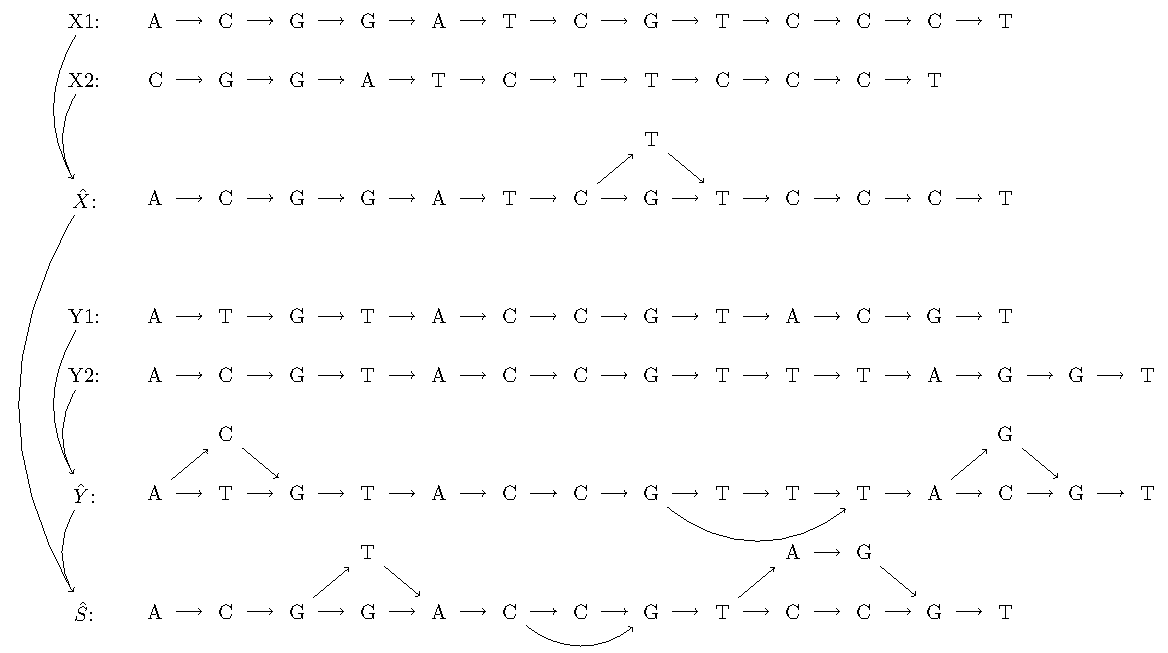
\includegraphics[width=\textwidth]{figures/graph_msa}

  \caption{
    Iterative sequence graph alignments of four sequences evolved in two generations from $S=\emph{ACGTACGTACGT}$.
    The sequences are represented as linear sequence graphs (X1, X2, Y1, Y2) and pairwise alignment is performed on the closest pairs yielding two sequence graphs ($\hat{X}, \hat{Y}$).
    These two sequence graphs are then aligned to each other, yielding a sequence graph representing an alignment of the two closest paths in the graphs ($\hat{S}$).
    As seen the original sequence is in the language of the final sequence graph}
  \label{fig:treealign}
\end{figure}

The sequence graph alignment algorithm can also be adapted to find the substring of a sequence graph $G_R$ that minimizes the edit distance to a sequence $Q$.
This solves the problem of mapping a read to a graph, which will be discussed further in section~\ref{sec:graphmapping}.


%%% Local Variables:
%%% mode: latex
%%% TeX-master: "main"
%%% End:
